\chapter{自动化安装系统}


Redhat系主要有两种方式安装系统Kickstart和Cobbler。
Kickstart是一种无人值守的安装方式。它的工作原理是在安装过程中记录人工干预填写的各种参数,并生成一个名为ks.cfg的文件。如果在自动安装过程中出现要填写参数的情况,安装程序首先会去查找ks.cfg文件,如果找到合适的参数,就采用所找到的参数;如果没有找到合适的参数,便会弹出对话框让安装者手工填写。所以,如果ks.cfg文件涵盖了安装过程中所有需要填写的参数,那么安装者完全可以只告诉安装程序从何处下载ks.cfg文件,然后就去忙自己的事情。等安装完毕,安装程序会根据ks.cfg中的设置重启/关闭系统,并结束安装。

Cobbler集中和简化了通过网络安装操作系统需要使用到的DHCP、TFTP和DNS服务的配置。Cobbler不仅有一个命令行界面,还提供了一个Web界面,大大降低了使用者的入门水平。Cobbler内置了一个轻量级配置管理系统,但它也支持和其它配置管理系统集成,如Puppet,暂时不支持SaltStack。

在这之前需要了解几个概念,PXE(pre-boot execution environment) 预启动执行环境,通过网络接口启动计算机,不依赖本地存储设备或本地已安装的操作系统,它的工作模式是client/server工作模式,PXE客户端会调用网际协议IP,用户数据报协议(UDP),动态主机设定(DHCP),小型文件传输协议(TFTP)等网络协议。
PXE工作过程

DHCP(Dynamic Host Configuration Protocol,动态主机配置协议)通常被应用在大型的局域网络环境中,主要作用是集中的管理、分配IP地址,使网络环境中的主机动态的获得IP地址、网关地址、DNS服务器地址等信息,并能够提升地址的使用率。端口号67,安装系统时开启,安装后关闭

 TFTP(Trivial File Transfer Protocol,简单文件传输协议)是TCP/IP协议族中的一个用来在客户机与服务器之间进行简单文件传输的协议,提供不复杂、开销不大的文件传输服务。端口号为69。

\ref{Fig:pxe-step}

\begin{enumerate}
\item PXE客户端(需要安装系统的机子) 通过PXE BOOTROM(自启动芯片)会以UDP发送一个广播,向本网络中的DHCP服务器索取IP
\item DHCP服务端收到客户端的请求,验证是否来至合法的PXE clinet的请求,验证通过它将给客户端一个响应其中包含为客户端分配的IP地址,PXELINUX启动程序(TFTP)位置以及配置文件所在位置
\item 客户端收到服务端的回应后会再请求传送启动所需文件:pxelinux.0, pxelinux.cfg/default. vmlinuz, initrd.img
\item 服务端通过TFTP通讯协议从Boot server下载启动安装程序所必需的文件,然后根据该文件中定义的引导顺序,启动linux安装程序的引导内核
\item 客户端通过pxelinux.cfg/default文件成功引导linux安装内核后,安装程序必须确定通过什么安装介质来安装linux,如果通过网络安培(nfs,ftp,http,),便会初始化网络,并定位安装源位置。此时会读取default文件中指定的自动应答文件ks.cfg所在位置,根据该位置请求下载该文件
\item 从服务端下载完ks.cfg文件后,通过该文件找到os server,并按照文件的配置请求下载安装过程需要的软件包。os server 和客户端建立连接后,将开始传输软件包,客户端将开始安装操作系统。安装完成后将重新引导计算机。
\end{enumerate}

这里有个问题,在第2步和第5步初始化2次网络了,这是由于PXE获取的是安装用的内核以及安装程序等,而安装程序要获取的是安装系统所需的二进制包以及配置文件。因此PXE模块和安装程序是相对独立的,PXE的网络配置并不能传递给安装程序,从而进行两次获取IP地址过程,但IP地址在DHCP的租期内是一样的。

\section{kickstart 安装部署步骤}
服务端环境环境:CentOS release 6.7 (Final)  ip 10.0.0.151 ,selinux,防火墙关闭, 首先安装DHCP,TFTP, HTTP服务

\lstinputlisting{./cobble/codes/installDhcp.sh}

好吧让我们来看看效果如果出现下面画面证明配置成功啦

\ref{Fig:kickstartDhcp}

配置支持PXE的启动程序 syslinux
syslinux是一个功能强大的引导加载程序,而且兼容各种介质。SYSLINUX是一个小型的Linux操作系统,它的目的是简化首次安装Linux的时间,并建立修护或其它特殊用途的启动盘。如果没有找到pxelinux.0这个文件,可以安装一下。

\lstinputlisting{./cobble/codes/installSyslinux.sh}

\subsection{创建ks.cfg文件}
kickstart是为了避免安装操作系统的过程中的交互操作,只要定义好一个kickstar自动应答配置文件ks.cfg,并让安装程序知道该配置文件的位置,就可以在安装中读取配置文件来安装系统。

生成kickstaart配置文件的三种方法:

每安装好一台Centos机器,Centos安装程序都会创建一个kickstart配置文件,记录你的真实安装配置。如果你希望实现和某系统类似的安装,可以基于该系统的kickstart配置文件来生成你自己的kickstart配置文件。(生成的文件名字叫anaconda-ks.cfg位于/root/anaconda-ks.cfg)

Centos提供了一个图形化的kickstart配置工具。在任何一个安装好的Linux系统上运行该工具,就可以很容易地创建你自己的kickstart配置文件。kickstart配置工具命令为redhat-config-kickstart(RHEL3)或system-config-kickstart(RHEL4,RHEL5).网上有很多用CentOS桌面版生成ks文件的文章,如果有现成的系统就没什么可说。但没有现成的,也没有必要去用桌面版,命令行也很简单。

阅读kickstart配置文件的手册。用任何一个文本编辑器都可以创建你自己的kickstart配置文件。

ks.cfg 文件组成大致分为3段

命令段:键盘类型,语言,安装方式等系统的配置,有必选项和可选项,如果缺少某项必选项,安装时会中断并提示用户选择此项的选项

* 软件包段

语法基本可以写成

\begin{lstlisting}
%packages
@groupname:指定安装的包组
package_name:指定安装的包
-package_name:指定不安装的包
* 脚本段(可选)

%pre:安装系统前执行的命令或脚本(由于只依赖于启动镜像,支持的命令很少)
%post:安装系统后执行的命令或脚本(基本支持所有命令)
\end{lstlisting}

首先要使用grub-crypt生成一个密码用于root密码,编写ks配置文件放到/var/www/html/ks_config/CentOS-6.7-ks.cfg,

%\lstinputlisting{./codes/cobble/CentOS-6.7-ks.cfg}

优化脚本,也需要放在下面。/var/www/html/ks_config/optimization.sh

%\lstinputlisting{./codes/cobble/optimization.sh}

编辑default配置文件

\begin{lstlisting}
 vim /var/lib/tftpboot/pxelinux.cfg/default
default ks
prompt 0
label ks
 kernel vmlinuz
 append initrd=initrd.img ks=http://10.0.0.151/ks_config/CentOS-6.7-ks.cfg # 告诉安装程序ks.cfg文件在哪里
# append initrd=initrd.img ks=http://10.0.0.151/ks_config/CentOS-6.7-ks.cfg ksdevice=eth0
# 多了一个参数是为了指定网卡(用于多块多卡的时候)
\end{lstlisting}

知识扩展
PXE配置文件default
由于多个客户端可以从一个PXE服务器引导,PXE引导映像使用了一个复杂的配置文件搜索方式来查找针对客户机的配置文件。如果客户机的网卡的MAC地址为8F:3H:AA:6B:CC:5D,对应的IP地址为10.0.0.195,那么客户机首先尝试以MAC地址为文件名匹配的配置文件,如果不存在就以IP地址来查找。根据上述环境针对这台主机要查找的以一个配置文件就是 /tftpboot/pxelinux.cfg/01-8F:3H:AA:6B:CC:5D。如果该文件不存在,就会根据IP地址来查找配置文件了,这个算法更复杂些,PXE映像查找会根据IP地址16进制命名的客户机配置文件。例如:10.0.0.195对应的16进制的形式为C0A801C3。(可以通过syslinux软件包提供的gethostip命令将10进制的IP转换为16进制)
如果C0A801C3文件不存在,就尝试查找C0A801C文件,如果C0A801C也不存在,那么就尝试C0A801文件,依次类推,直到查找C文件,如果C也不存在的话,那么最后尝试default文件。
总体来说,pxelinux搜索的文件的顺序是:

\begin{lstlisting}
/tftpboot/pxelinux.cfg/01-88-99-aa-bb-cc-dd
/tftpboot/pxelinux.cfg/C0A801C3
/tftpboot/pxelinux.cfg/C0A801C
/tftpboot/pxelinux.cfg/C0A801
/tftpboot/pxelinux.cfg/C0A80
/tftpboot/pxelinux.cfg/C0A8
/tftpboot/pxelinux.cfg/C0A
/tftpboot/pxelinux.cfg/C0
/tftpboot/pxelinux.cfg/C
/tftpboot/pxelinux.cfg/default
\end{lstlisting}


\section{Cobbler}

yum install dhcp tftp-server xinetd httpd cobbler cobbler-web pykickstart –y

\begin{figure}[!ht]
    \centering
     \caption{\label{Fig:pxe-step} pxe step}
    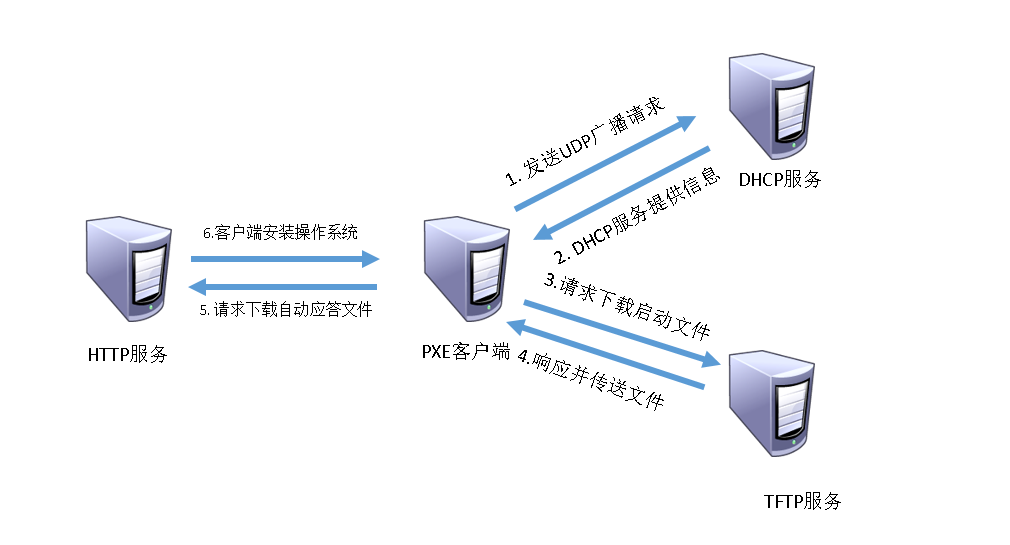
\includegraphics[width=0.8\textwidth]{./cobble/images/pxe-step.png}
\end{figure}

\begin{figure}[!ht]
    \centering
     \caption{\label{Fig:kickstart-dhcp} pxe step}
    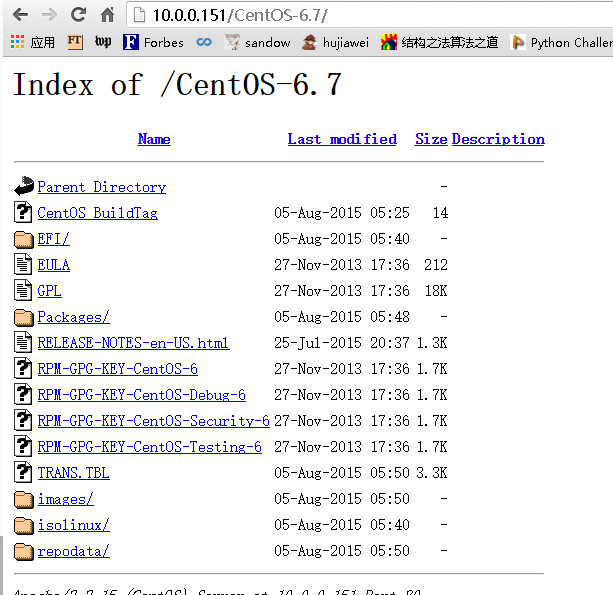
\includegraphics[width=0.8\textwidth]{./cobble/images/kickstart-dhcp.png}
\end{figure}

kickstart https://access.redhat.com/documentation/en-us/red_hat_enterprise_linux/6/html/installation_guide/s1-kickstart2-options
